\pdfminorversion=7
\documentclass{article}

% NeurIPS submission style. Keep the default option for double-blind review.
\usepackage{neurips_2026}

\usepackage[utf8]{inputenc}
\usepackage[T1]{fontenc}
\usepackage{hyperref}
\usepackage{url}
\usepackage{booktabs}
\usepackage{amsfonts}
\usepackage{amsmath}
\usepackage{amsthm}
\usepackage{nicefrac}
\usepackage{microtype}
\usepackage{xcolor}
\usepackage{graphicx}
\usepackage{array}

\title{Pandora-RAG: Adaptive Stopping for Multi-Hop Retrieval with Anytime-Valid Risk Monitoring}

\author{Anonymous Authors}

\newcommand{\method}{Pandora-RAG}
\newcommand{\hotpot}{HotpotQA}
\newcommand{\musique}{MuSiQue}
\newcommand{\twowiki}{2WikiMultiHopQA}
\newtheorem{proposition}{Proposition}[section]

\begin{document}

\maketitle

\begin{abstract}
Iterative multi-hop retrieval can uncover bridge evidence for complex question answering, but each additional retrieval step increases latency and may introduce distractors. We study when a RAG system should stop retrieving. \method{} formulates iterative retrieval as a fixed-order finite-horizon optimal stopping problem, derives a Bellman oracle from fully rolled-out trajectories, and uses this oracle both as a structural upper bound and as supervision for stop/continue decisions. Because oracle answer quality is not observable at deployment time, \method{} trains a lightweight neural probe from LLM hidden states and observable retrieval features, and then selects cost-aware per-step stopping thresholds on development data. To make the resulting adaptively stopped stream monitorable, \method{} attaches an outcome-aware E-value process for delayed-feedback or audited streams, providing anytime-valid evidence against a low-error-rate null without asserting label-free real-time safety or strict empirical error-rate control. On \hotpot{}, \musique{}, and \twowiki{}, the probe recovers 79.9--85.4\% of oracle F1 while using only 1.73--3.31 retrieval steps on average, yielding a low-retrieval Pareto operating point rather than uniformly maximizing F1. Adding the E-value monitor changes average retrieval depth by only 0.5--6.4\% relative to the probe and preserves or improves F1 on two of the three datasets. Under an aligned fixed-checkpoint online threshold sweep, \method{} achieves higher F1 and EM than Stop-RAG with fewer retrieval steps on all three benchmarks.
\end{abstract}

\section{Introduction}

Retrieval-augmented generation (RAG) improves knowledge-intensive NLP by coupling parametric language models with external evidence \citep{lewisRetrievalAugmentedGenerationKnowledgeIntensive2020}. For complex multi-hop questions, retrieval is often iterative rather than one-shot: systems alternate between partial reasoning and additional evidence acquisition, as in IRCoT, Iter-RetGen, and Self-RAG \citep{trivediInterleavingRetrievalChainofThought2023,shaoEnhancingRetrievalAugmentedLarge2023,asaiSelfRAGLearningRetrieve2023}. This iterative structure creates a deployment dilemma. One more retrieval step may uncover the bridge fact needed for the answer, but it also increases latency, token cost, and the chance of introducing distractors. The value of continuing is therefore highly instance-dependent.

Recent adaptive RAG methods recognize this heterogeneity, but most of them decide whether retrieval is needed, which reasoning strategy should be selected, or whether the current state appears uncertain \citep{jeongAdaptiveRAGLearningAdapt2024a,baekProbingRAGSelfProbingGuide2025,yaoSeaKRSelfawareKnowledge2025}. Stop-RAG is closest to our setting because it learns a value-based controller for iterative retrieval \citep{parkStopRAGValueBasedRetrieval2025}. Nevertheless, two issues remain insufficiently separated. First, sequential retrieval has a clear fixed-order stopping structure, yet deployed policies are often evaluated without an explicit oracle upper bound tied to the realized trajectory. Second, once stopping is adaptive, deployment requires more than an offline accuracy estimate; it also requires an online signal indicating whether the stopped-answer stream is entering a high-risk regime.

We address the first issue by framing iterative multi-hop RAG as a finite-horizon fixed-order optimal stopping problem. This framing is inspired by Pandora-style costly information acquisition \citep{weitzmanOptimalSearchBest1979,gergatsouliWeitzmansRulePandoras2023,atsidakouContextualPandorasBox2024}, but it differs in an important respect: multi-hop retrieval is state-dependent because the distribution of the next retrieved document depends on the evidence already observed. The formal object is therefore a Bellman stopping recursion over realized RAG states, rather than an assumption that classical independent-box reservation values apply without modification.

This perspective yields a three-layer design. First, we compute a Bellman oracle from fully rolled-out trajectories and use it both as a structural upper bound and as supervision for stop/continue decisions. Second, because answer quality is not observable at deployment time, we train a lightweight neural probe from LLM hidden states and inexpensive observable retrieval features. Third, we attach an E-value process to the adaptively stopped stream when delayed or audited outcomes become available. E-values and safe testing provide evidence that remains valid under optional continuation \citep{shaferTestingBettingStrategy2021,grunwaldSafeTesting2024}. In our setting, the monitor is not intended to enforce strict empirical risk control or provide a label-free real-time guarantee; instead, it supplies anytime-valid evidence against a low-error-rate null for deployment streams with outcome feedback, complementing conformal and uncertainty-aware approaches for RAG reliability \citep{angelopoulosConformalRiskControl2024,chakrabortyPrincipledContextEngineering2026,fengResponseQualityAssessment2025}.

Our contributions are threefold. First, we formulate iterative multi-hop RAG stopping as a fixed-order sequential information-acquisition problem and use a Bellman oracle as both an upper bound and a source of supervision. Second, we train a deployable stopping probe and audit a Lite variant with normalized cost accounting, thereby separating retrieval and generation cost from stopping-feature overhead. Third, we attach an E-value process to the adaptively stopped stream, which yields an online risk-evidence trace when stopped-answer outcomes are later revealed through labels, review, corrections, or factuality audits. Empirically, on \hotpot{}, \musique{}, and \twowiki{}, the learned probe recovers 79.9--85.4\% of the oracle F1 while operating far below full fixed-depth retrieval; it is a cost-aware operating point rather than a uniformly best-F1 policy. Under an aligned fixed-checkpoint online threshold sweep, \method{} remains above the Stop-RAG frontier in F1/EM versus average retrieval depth.

\section{Related Work}
\label{sec:related}

\paragraph{Iterative and adaptive retrieval for RAG.}
RAG introduced the standard retrieve-and-generate formulation for knowledge-intensive NLP \citep{lewisRetrievalAugmentedGenerationKnowledgeIntensive2020}. Later work made retrieval iterative or tightly interleaved retrieval with reasoning, including IRCoT, Iter-RetGen, and Self-RAG \citep{trivediInterleavingRetrievalChainofThought2023,shaoEnhancingRetrievalAugmentedLarge2023,asaiSelfRAGLearningRetrieve2023}. Adaptive-RAG routes queries across strategies based on predicted complexity \citep{jeongAdaptiveRAGLearningAdapt2024a}; Probing-RAG and SeaKR use internal states or uncertainty to decide whether and how to retrieve \citep{baekProbingRAGSelfProbingGuide2025,yaoSeaKRSelfawareKnowledge2025}; and Stop-RAG learns a value-based controller for iterative retrieval depth \citep{parkStopRAGValueBasedRetrieval2025}. Our setting is closest to Stop-RAG, but our emphasis is different: we explicitly separate a Bellman oracle upper bound from the deployable policy, and we add a monitoring layer for the adaptively stopped stream.

\paragraph{Optimal stopping, Pandora-style search, and metareasoning.}
Classical Pandora-style search studies costly sequential information acquisition and yields threshold-style optimal policies under structural assumptions \citep{weitzmanOptimalSearchBest1979}. Recent work extends this view to correlated and contextual settings \citep{chawlaPandorasBoxCorrelations2020,gergatsouliWeitzmansRulePandoras2023,atsidakouContextualPandorasBox2024}, while rational metareasoning connects computation-time decisions to utility-aware control in language models \citep{sabbataRationalMetareasoningLarge2025}. \method{} is motivated by this literature but does not assume that multi-hop retrieval satisfies the independent-box model. Instead, we use a fixed-order finite-horizon Bellman recursion that permits state dependence, and we treat Pandora-style search as a structural analogy rather than a theorem applied verbatim.

\paragraph{Risk control and uncertainty for RAG.}
Conformal Risk Control generalizes split conformal prediction from coverage to expected losses \citep{angelopoulosConformalRiskControl2024}, and recent RAG-specific work uses conformal prediction or factuality calibration to control context selection or answer quality \citep{chakrabortyPrincipledContextEngineering2026,fengResponseQualityAssessment2025}. URAG highlights the broader need for uncertainty evaluation in RAG systems \citep{nguyenURAGBenchmarkUncertainty2026}. Our monitor is complementary to these methods: rather than offering a static marginal guarantee for a calibrated predictor, it maintains sequential E-value evidence on the stream produced by an adaptively stopped system \citep{shaferTestingBettingStrategy2021,grunwaldSafeTesting2024}.

\paragraph{Cost-aware routing and cascades.}
A separate line of work optimizes cost-performance tradeoffs by routing among models or cascades, as in FrugalGPT, MixLLM, C3PO, and CCPO \citep{chenFrugalGPTHowUse2023,wangMixLLMDynamicRouting2025a,valkanasC3POOptimizedLarge2025,siConformalConstrainedPolicy2026}. These methods address a related but distinct problem: choosing which model or policy to invoke. We instead study whether to continue retrieving within a fixed iterative multi-hop RAG trajectory.

\section{Method}
\label{sec:method}

Figure~\ref{fig:method-overview} summarizes the full pipeline. We first roll out each training example to the maximum depth and construct Bellman stop/continue labels from the realized trajectory. We then train a deployable neural probe from hidden states and observable step features, and select its operating point on development data under a cost-aware budget. Finally, an outcome-aware E-value process monitors the stopped-answer stream produced by the probe in delayed-feedback or audited deployments. The oracle uses future realized quality only for supervision and upper-bound analysis, whereas the E-value layer monitors the stopped stream rather than directly revising answers.

\begin{figure}[t]
  \centering
  \includegraphics[width=\linewidth]{figs/architechture.pdf}
  \caption{Overview of \method{}. Full rollouts are used only offline to derive Bellman oracle labels and train the stopping probe. At deployment, the probe decides whether to continue retrieval from hidden and observable state features, and the E-value layer monitors the adaptively stopped answer stream for low-risk violations once delayed or audited outcomes are revealed.}
  \label{fig:method-overview}
\end{figure}

\subsection{Fixed-order stopping for iterative RAG}
\label{sec:problem}

For a question $q$, an iterative RAG system produces a fixed-order sequence of retrieval states
\[
  s_k=(q,d_{1:k},a_k,\phi_k), \qquad k=1,\ldots,K,
\]
where $d_{1:k}$ are the documents retrieved so far, $a_k$ is the current answer, and $\phi_k$ denotes observable step features such as retrieval scores, answer-confidence proxies, answer-change features, and cost logs. Let $\mathcal{F}_k=\sigma(s_1,\ldots,s_k)$ denote the information available after step $k$. A stopping policy chooses a stopping time $\tau\in\{1,\ldots,K\}$ with respect to this filtration and returns $a_\tau$.

Let $Q(s_k)\in[0,1]$ denote the answer quality at step $k$; in experiments, we use token-level F1 for the stopping oracle and also report exact match. Let $c_k\ge 0$ be the cost of executing retrieval/generation step $k$. The cost-quality objective is
\begin{equation}
  J(\pi)
  =
  \mathbb{E}_{\pi}\left[
    Q(s_{\tau_\pi})-\sum_{j=1}^{\tau_\pi}c_j
  \right].
  \label{eq:utility}
\end{equation}
This formulation separates the decision problem from the retrieval order: the retriever and generator define the ordered trajectory, while \method{} learns when to stop along that trajectory. The main experiments use a fixed per-step oracle cost and report average retrieval steps as the primary cost metric; the implementation also supports token-weighted and latency-weighted costs.

\subsection{Bellman oracle and supervision}
\label{sec:bellman-oracle}

In the population problem, finite-horizon optimal stopping admits the Bellman recursion
\begin{align}
  V_K^*(s_K) &= Q(s_K), \\
  V_k^*(s_k) &=
  \max\left\{
    Q(s_k),
    \mathbb{E}\left[V_{k+1}^*(s_{k+1})\mid\mathcal{F}_k\right]-c_{k+1}
  \right\},
  \qquad k<K .
  \label{eq:bellman}
\end{align}
The optimal action compares the value of stopping immediately with the value of continuing. Defining
\[
  \Delta_k^*(s_k)=
  \mathbb{E}\left[V_{k+1}^*(s_{k+1})\mid\mathcal{F}_k\right]
  -c_{k+1}-Q(s_k),
\]
the oracle continues when $\Delta_k^*(s_k)>0$ and stops otherwise. This fixed-order structure motivates the name \method{}: as in Pandora-style search, the system asks whether observing one more information source is worth its cost. Unlike the classical independent-box setting, however, multi-hop retrieval is state-dependent because the next retrieval distribution depends on the evidence already found. Our deployable method therefore relies on the Bellman fixed-order recursion rather than claiming to learn exact Weitzman reservation values.

Stage 1 constructs a trajectory-level oracle by forcing each example to run to $K$ and then applying backward dynamic programming to the realized qualities. For example $i$, let $Q_k^i=Q(s_k^i)$ and $c_k^i$ be the observed quality and cost at step $k$. We compute
\begin{equation}
  \widetilde V_K^i=Q_K^i,\qquad
  \widetilde V_k^i=\max\left\{Q_k^i,\widetilde V_{k+1}^i-c_{k+1}^i\right\}.
  \label{eq:trajectory-dp}
\end{equation}
The oracle stops at the first $k$ such that
\[
  Q_k^i \ge \widetilde V_{k+1}^i-c_{k+1}^i,
\]
or at $K$ if no earlier step satisfies the inequality. It also provides step-level training labels
\begin{equation}
  m_k^i=(\widetilde V_{k+1}^i-c_{k+1}^i)-Q_k^i,
  \qquad
  y_k^i=\mathbb{I}\{m_k^i>0\},
  \label{eq:oracle-labels}
\end{equation}
where $m_k^i$ is the continuation margin and $y_k^i=1$ denotes \textsc{Continue}. This oracle is not deployable because it uses future realized answer quality, but it serves two roles: it provides an upper bound for the chosen RAG trajectory and supplies supervision for a deployable stopping signal.

Appendix~\ref{app:proofs} states the assumptions and provides complete proofs for the Bellman recursion, the realized-trajectory dynamic program, and the E-process guarantee used later in Section~\ref{sec:evalue-method}.

\subsection{Neural stopping probe}
\label{sec:probe}

At deployment time, neither $Q(s_k)$ nor the future trajectory is observed. \method{} therefore learns a continuation-decision estimator from observable state representations. For each step, the probe input is
\[
  x_k=(h_k,\phi_k),
\]
where $h_k$ is the last-layer hidden representation of the generator state and $\phi_k$ is the shallow feature vector. The main probe is a two-branch MLP: a hidden branch normalizes and compresses $h_k$, a shallow branch embeds $\phi_k$, and a fusion head maps the concatenated representation to a continuation logit. A Lite variant removes higher-overhead features such as uncertainty and consistency scores, while retaining hidden states, step and retrieval-score features, token/latency logs, and inexpensive lexical stability features for deployment-cost auditing.

The probe predicts
\begin{equation}
  p_\theta(k)=\Pr_\theta(y_k=1\mid x_k),
  \label{eq:probe-prob}
\end{equation}
where $y_k$ is the oracle continuation label from Eq.~\eqref{eq:oracle-labels}. We train the probe with focal binary cross-entropy, label smoothing, dropout, weight decay, and early stopping. Abstractly, the objective is
\begin{equation}
  \mathcal{L}_{\mathrm{probe}}(\theta)
  =
  \mathbb{E}\left[
    w_k\,
    \ell_{\mathrm{focal}}\left(p_\theta(k),y_k\right)
  \right],
  \label{eq:probe-loss}
\end{equation}
where $w_k$ can emphasize high-margin oracle decisions. We use binary continuation labels as the main supervision because F1-regression heads consistently underperformed in policy evaluation.

The deployed stopping rule uses per-step thresholds $\eta_k$:
\begin{equation}
  \hat a_k=
  \begin{cases}
    \textsc{Continue}, & p_\theta(k)\ge \eta_k \text{ and } k<K,\\
    \textsc{Stop}, & p_\theta(k)<\eta_k \text{ or } k=K .
  \end{cases}
  \label{eq:probe-policy}
\end{equation}
Thresholds are selected on the development split. Candidate policies must remain within a development-step budget tied to the Global-Weitzman structural reference; among feasible policies, we maximize a cost-aware utility of the form $\mathrm{F1}-\lambda\cdot\mathrm{normalized\ cost}$. A conservative per-step refinement is accepted only if it improves the development utility, matched-budget F1, or the Pareto frontier. The reported probe is therefore a budget-aware operating point rather than a pure max-F1 classifier.

\subsection{E-value risk monitor}
\label{sec:evalue-method}

The learned probe remains an imperfect adaptive stopper. \method{} therefore adds a monitoring layer over the stream of stopped answers. The monitor is intended for delayed-feedback or audited deployment streams, where stopped-answer outcomes are eventually revealed by benchmark labels, human review, user correction, or post-hoc factuality assessment. It is not a label-free real-time safety guarantee. Fix a quality threshold $\gamma$ and nominal error level $\alpha$. For the $n$th deployment example, after the policy stops at $\tau_n$ and its outcome is revealed, define
\[
  e_n=\mathbb{I}\{Q(s_{\tau_n})<\gamma\}.
\]
The monitor tests the low-risk null
\begin{equation}
  H_0:\quad
  \mathbb{E}[e_n\mid\mathcal{G}_{n-1}]\le \alpha
  \quad\text{for all }n,
  \label{eq:low-risk-null}
\end{equation}
where $\mathcal{G}_{n-1}$ is the pre-outcome information available before the $n$th outcome is revealed, including previous examples, previous audited outcomes, and the current candidate-stop features. This null concerns the adaptively stopped system as deployed; it is not an assumption that the test stream is i.i.d.

Before updating the E-process, we train a light quality model on the calibration split,
\[
  \hat p_n
  =
  \Pr_\psi\!\left(Q(s_{\tau_n})\ge\gamma
  \mid z_{\tau_n},p_\theta(\tau_n)\right),
\]
where $z_{\tau_n}$ contains shallow quality features and the probe continuation probability. In the current implementation, this model is a standardized logistic regression with class-balanced loss. A calibration quantile defines a quality bar: when the probe proposes stopping at a candidate step for which $\hat p$ falls below the bar, the monitored policy delays stopping when possible. The same quality estimate also sets a predictable betting fraction
\[
  \lambda_n=\operatorname{clip}(1-\hat p_n,\epsilon,1-\epsilon).
\]
The outcome-aware E-value update is
\begin{equation}
  E_0=1,\qquad
  E_n=E_{n-1}\left(1-\lambda_n+\lambda_n\frac{e_n}{\alpha}\right).
  \label{eq:evalue-update}
\end{equation}
Because $\lambda_n$ is predictable with respect to $\mathcal{G}_{n-1}$, Eq.~\eqref{eq:low-risk-null} implies that $(E_n)$ is a nonnegative supermartingale under $H_0$. The standard Ville inequality gives the anytime-valid alarm guarantee
\begin{equation}
  \Pr_{H_0}\left(\sup_n E_n\ge 1/\delta\right)\le \delta .
  \label{eq:ville}
\end{equation}
In experiments, we report wealth capped at the operational boundary $1/\alpha$ and use boundary crossing as risk evidence or, in the selective-prediction variant, as a trigger for abstention. The E-value layer is a monitor rather than an optimizer: it can detect sustained risk under adaptive stopping and distribution shift once outcome feedback is available, but it does not by itself guarantee that the realized empirical error rate is below $\alpha$.

\section{Experimental setup}
\label{sec:setup}

\paragraph{Tasks and splits.}
We evaluate on three multi-hop question answering benchmarks: \hotpot{} \citep{yangHotpotQADatasetDiverse2018}, \musique{} \citep{trivediMuSiQueMultihopQuestions2022}, and \twowiki{} \citep{hoConstructingMultihopQADataset2020}. Each dataset is divided into disjoint train, calibration, development, and test partitions with seed 42. The calibration split is reserved for Stage-3 quality-model calibration, E-value and CP calibration, and betting-related thresholds. The development split is used for Stage-2 stopping-threshold selection. Test examples are used only for final evaluation.

\begin{table}[t]
  \caption{Datasets and deterministic splits. \musique{} has fewer test examples because the default quota reserves calibration and development examples from the available validation pool.}
  \label{tab:splits}
  \centering
  \small
  \begin{tabular}{llrrrrr}
    \toprule
    Dataset & Hop type & Train & Calib & Dev & Test & Seed \\
    \midrule
    \hotpot{} & 2-hop distractor QA & 4000 & 1000 & 1000 & 1000 & 42 \\
    \musique{} & 2--4 hop QA & 4000 & 1000 & 1000 & 417 & 42 \\
    \twowiki{} & multi-entity multi-hop QA & 4000 & 1000 & 1000 & 1000 & 42 \\
    \bottomrule
  \end{tabular}
\end{table}

\paragraph{RAG backbone and trajectories.}
Each example is processed by a fixed-order iterative RAG pipeline with maximum retrieval depth $K=5$. At each step, the system records the retrieved document, retrieval score, current answer, answer F1 and exact match against the gold answer, shallow observable features, and LLM hidden states for the current cumulative state. The model used for generation and state encoding is Llama-3.1-8B-Instruct with deterministic generation. The main hidden representation is the last-layer, last-token vector of dimension 4096, extracted separately for each retrieval step so that the representation is aligned with step-level stopping labels.

\paragraph{Trajectory annotation.}
Fully rolled-out trajectories are annotated with the Bellman labels described in Section~\ref{sec:bellman-oracle}. The oracle uses the realized per-step F1 values and a fixed per-step cost in the main record. These labels are used only for supervision and upper-bound reporting; all deployed policies in the main comparison choose their stopping step from observable state features.

\paragraph{Baselines and metrics.}
We compare against fixed-depth retrieval for $K\in\{1,2,3,4,5\}$, a deployable static Weitzman proxy, an F1-based Global-Weitzman structural reference, an instance-level dynamic-programming oracle, the learned Probe without monitoring, Probe+E-value, Probe+CP, and an aligned fixed-checkpoint online threshold sweep of Stop-RAG \citep{parkStopRAGValueBasedRetrieval2025}. Answer quality is measured by token-level F1 and exact match (EM), and retrieval cost is summarized by average retrieval steps. For risk monitoring, we report the error rate at threshold $\gamma$, final E-wealth, whether the E-process reaches its boundary, and selective-prediction coverage/accuracy when abstention is enabled.

Appendix~\ref{app:repro} records the deterministic split manifests, code-bundle entry points, and artifact-producing scripts used in the paper. Appendix~\ref{app:stage2}, Appendix~\ref{app:stage3}, and Appendix~\ref{app:stoprag-supp} collect the extended operating-point, robustness, and matched-budget comparison tables referenced throughout Sections~\ref{sec:results} and~\ref{sec:ablations}.

\section{Results}
\label{sec:results}

\subsection{Adaptive stopping provides a low-cost Pareto point}
\label{sec:adaptive-results}

Table~\ref{tab:stage2-main} reports the fixed-depth baselines, a deployable static proxy, structural references, the oracle upper bound, and the learned probe. The oracle is not deployable because it uses realized answer quality along the full trajectory; it is included as an upper bound and as the source of supervision. The F1-Global-Weitzman row is also a structural reference: its reservations are estimated from training-set F1 gains, and its stopping decision compares against current realized F1 on the test trajectory, which is unavailable online. To audit the deployable version of the same static idea, Deployable-GW replaces F1 with an observable self-consistency proxy.

\begin{table}[t]
  \caption{Adaptive stopping results on the test set. The learned probe recovers most of the oracle benefit at low retrieval depth, but it does not uniformly outperform the best fixed depth on every dataset.}
  \label{tab:stage2-main}
  \centering
  \small
  \resizebox{\linewidth}{!}{
  \begin{tabular}{lrrrrrr}
    \toprule
    Strategy & \multicolumn{2}{c}{\hotpot{}} & \multicolumn{2}{c}{\musique{}} & \multicolumn{2}{c}{\twowiki{}} \\
    \cmidrule(lr){2-3}\cmidrule(lr){4-5}\cmidrule(lr){6-7}
    & F1 & Steps & F1 & Steps & F1 & Steps \\
    \midrule
    Fixed-K=1 & 0.4340 & 1.00 & 0.0797 & 1.00 & 0.2846 & 1.00 \\
    Fixed-K=2 & 0.6773 & 2.00 & 0.1830 & 2.00 & 0.5908 & 2.00 \\
    Fixed-K=3 & 0.6775 & 3.00 & 0.3210 & 3.00 & 0.5583 & 3.00 \\
    Fixed-K=4 & 0.6747 & 4.00 & 0.3816 & 4.00 & 0.5382 & 4.00 \\
    Fixed-K=5 & 0.6668 & 4.99 & 0.4022 & 5.00 & 0.5288 & 5.00 \\
    Deployable-GW & 0.4340 & 1.00 & 0.0797 & 1.00 & 0.2846 & 1.00 \\
    F1-Global-Weitzman & 0.7092 & 1.64 & 0.4229 & 3.29 & 0.6449 & 1.77 \\
    Oracle & 0.7810 & 1.58 & 0.4966 & 2.12 & 0.6954 & 1.59 \\
    Probe & 0.6544 & 1.73 & 0.3969 & 3.31 & 0.5941 & 1.82 \\
    \bottomrule
  \end{tabular}}
\end{table}

The key result is not that the learned probe always obtains the highest single-point F1. On \hotpot{}, the best fixed depth is $K=3$ with F1 0.6775, whereas Probe obtains 0.6544 at 1.73 steps. On \musique{}, Probe nearly matches the full-depth fixed baseline with 3.31 rather than 5.00 steps. On \twowiki{}, Probe slightly exceeds the best fixed depth while using fewer steps than $K=2$. The F1-based Global-Weitzman reference performs surprisingly well, showing that much of the value comes from global depth regularities when answer quality is visible. However, its deployable self-consistency version collapses to the first-step point on all three datasets. Across datasets, Probe recovers 83.8\%, 79.9\%, and 85.4\% of the oracle F1 on \hotpot{}, \musique{}, and \twowiki{}, respectively, while substantially outperforming Deployable-GW. This supports the intended claim: adaptive stopping is valuable as a cost-quality tradeoff and should be evaluated on the Pareto frontier rather than only as a max-F1 classifier.

We also audit the deployment overhead of the stopping features. Table~\ref{tab:lite-cost} compares the main probe with a Lite variant that removes expensive uncertainty and consistency features while retaining hidden states, step and retrieval-score features, token/latency logs, and inexpensive lexical stability features. Lite preserves nearly the same cost-quality point: F1 decreases by 0.001--0.009, while feature overhead decreases by about three quarters. Because retrieval and generation dominate the normalized cost model, the end-to-end cost reduction is more modest, ranging from 0.3\% to 5.7\%.

\begin{table}[t]
  \caption{Lite Probe deployment audit. Lite removes higher-overhead stopping features and preserves most of the cost-quality point of the main probe. Cost deltas use normalized accounting weights: retrieval $1.0$, generation $1.0$, Full features $0.08$, Lite features $0.02$, and probe forward $0.01$ per step.}
  \label{tab:lite-cost}
  \centering
  \small
  \resizebox{\linewidth}{!}{
  \begin{tabular}{lrrrrrr}
    \toprule
    Dataset & Full F1 & Full steps & Lite F1 & Lite steps & Lite/oracle F1 & Total cost $\Delta$ \\
    \midrule
    \hotpot{} & 0.6544 & 1.732 & 0.6531 & 1.682 & 83.6\% & -5.7\% \\
    \musique{} & 0.3969 & 3.305 & 0.3918 & 3.391 & 78.9\% & -0.3\% \\
    \twowiki{} & 0.5941 & 1.822 & 0.5855 & 1.829 & 84.2\% & -2.5\% \\
    \bottomrule
  \end{tabular}}
\end{table}

\begin{figure}[t]
  \centering
  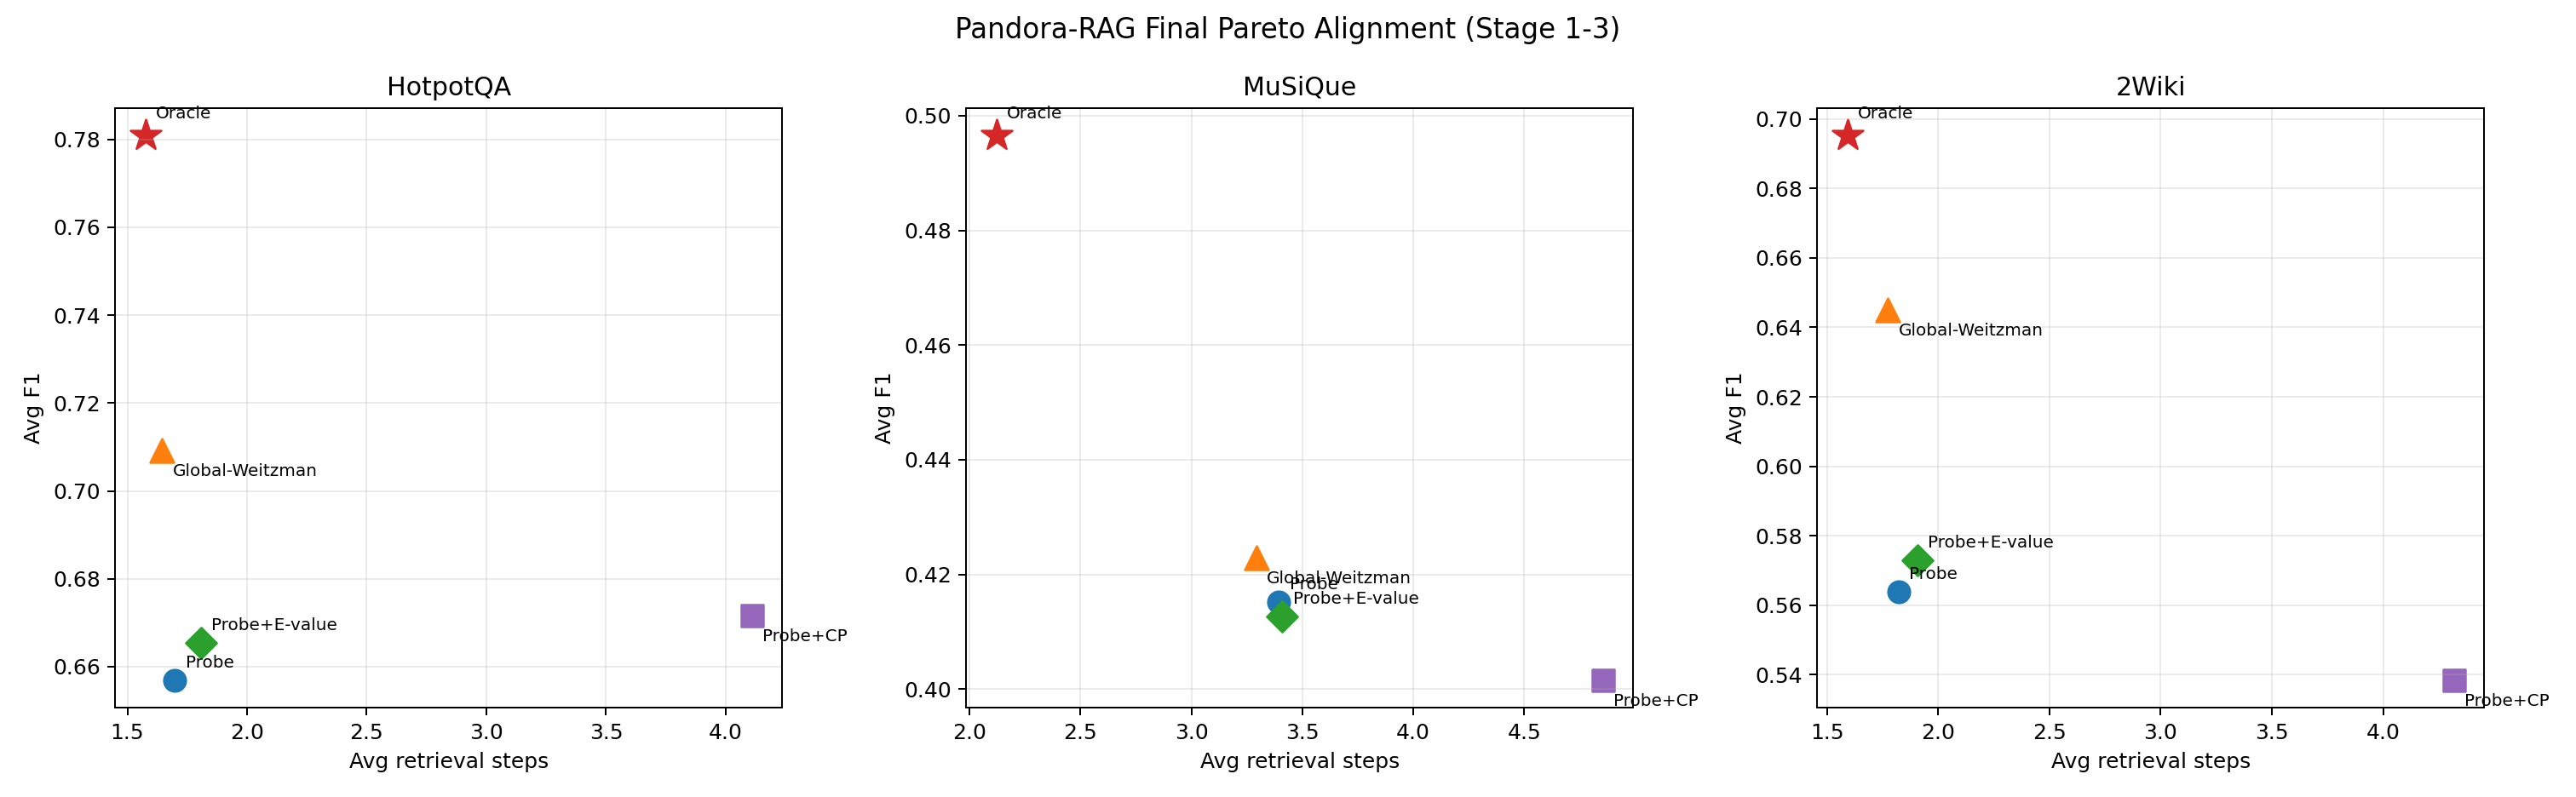
\includegraphics[width=0.92\linewidth]{results/stage3_final_pareto_all.png}
  \caption{F1 versus average retrieval steps for the oracle, structural baselines, Probe, Probe+E-value, and Probe+CP. Probe remains in the low-cost region; adding the E-value monitor produces only a small change in average steps, whereas CP moves the system toward substantially larger retrieval budgets.}
  \label{fig:pareto}
\end{figure}

\subsection{E-value monitoring adds little retrieval overhead}
\label{sec:evalue-main}

Table~\ref{tab:stage3-main} evaluates the risk-monitoring layer at $\gamma=0.5$ and $\alpha=0.1$ with predictive betting. The Probe rows here come from the monitor-compatible Stage-3 entry point rather than the standalone Stage-2 sweep in Table~\ref{tab:stage2-main}; small numeric differences are therefore expected. Probe+E-value preserves the low-cost character of the probe: average steps increase from 1.70 to 1.81 on \hotpot{}, from 3.39 to 3.41 on \musique{}, and from 1.82 to 1.91 on \twowiki{}. F1 improves slightly on \hotpot{} and \twowiki{} and remains essentially unchanged on \musique{}. In contrast, Probe+CP is substantially more expensive: it raises average steps to 4.11, 4.85, and 4.32, respectively, without uniform quality gains.

\begin{table}[t]
  \caption{Risk-monitoring results at $\gamma=0.5$ and $\alpha=0.1$. E-value monitoring has low overhead; CP is substantially more expensive and dataset-sensitive.}
  \label{tab:stage3-main}
  \centering
  \small
  \resizebox{\linewidth}{!}{
  \begin{tabular}{llrrrr}
    \toprule
    Dataset & Method & F1 & EM & Error rate & Steps \\
    \midrule
    \hotpot{} & Probe & 0.6569 & 0.5190 & 0.3030 & 1.70 \\
    \hotpot{} & Probe+E-value & 0.6654 & 0.5290 & 0.2950 & 1.81 \\
    \hotpot{} & Probe+CP & 0.6716 & 0.5310 & 0.2960 & 4.11 \\
    \midrule
    \musique{} & Probe & 0.4152 & 0.3189 & 0.5803 & 3.39 \\
    \musique{} & Probe+E-value & 0.4127 & 0.3141 & 0.5827 & 3.41 \\
    \musique{} & Probe+CP & 0.4015 & 0.3046 & 0.5971 & 4.85 \\
    \midrule
    \twowiki{} & Probe & 0.5639 & 0.4740 & 0.4090 & 1.82 \\
    \twowiki{} & Probe+E-value & 0.5728 & 0.4810 & 0.4010 & 1.91 \\
    \twowiki{} & Probe+CP & 0.5383 & 0.4340 & 0.4370 & 4.32 \\
    \bottomrule
  \end{tabular}}
\end{table}

The E-wealth traces should be interpreted as online risk evidence, not as a mechanism that enforces an empirical error rate below $\alpha$. Let $e_t=\mathbf{1}\{\mathrm{F1}_t<\gamma\}$ be the error indicator for the stopped answer at time $t$. The monitor tests the low-risk null
\[
H_0:\mathbb{E}[e_t\mid \mathcal{G}_{t-1}]\le \alpha,
\]
using predictable betting fractions $\lambda_t$ and the E-process
\[
E_n=\prod_{t=1}^{n}\left(1-\lambda_t+\lambda_t e_t/\alpha\right),
\qquad
\Pr_{H_0}\left(\sup_n E_n\ge 1/\delta\right)\le \delta.
\]
Under the no-shift main evaluation at $\alpha=0.1$, final E-wealth is 0.014 on \hotpot{}, 4.193 on \musique{}, and 10.000 on \twowiki{}, with reported wealth capped at $1/\alpha=10$. Thus, \twowiki{} reaches the alarm boundary, \musique{} accumulates risk evidence without reaching the cap, and \hotpot{} acts primarily as a low-cost quality gate in this configuration.

\subsection{Risk evidence responds to degraded streams}
\label{sec:shift}

We further evaluate test-time streams with sudden, gradual, and periodic distribution shifts. These shifts reorder the test stream so that more difficult examples become concentrated or repeated later in the sequence. The stable finding is that E-value wealth is sensitive to clearly degraded streams, especially for \musique{} and \twowiki{}. Under sudden shift, all three datasets reach the cap at $\alpha=0.1$; at $\alpha=0.2$, \musique{} and \twowiki{} still trigger reliably, whereas \hotpot{} is more dependent on the precise shift path. Under gradual and periodic shifts, \musique{} and \twowiki{} again show strong responses across $\alpha\in\{0.1,0.2\}$, whereas \hotpot{} responds mainly at $\alpha=0.1$.

This behavior reflects the intended role of the monitor. The E-process provides an online trajectory of risk evidence for the adaptively stopped system. A fixed CP threshold, by contrast, is calibrated before deployment and does not by itself create a sequential alarm that reacts to a changing test stream.

Figure~\ref{fig:evalue-shift-evidence} shows a representative \hotpot{} case at $\alpha=0.1$ and $\gamma=0.5$. Under no shift, the E-wealth trace stays far below the rejection boundary for most of the stream; under sudden shift, the same monitor climbs to the boundary shortly after the stream becomes more difficult. The cumulative error curve exposes the stream degradation, while the E-process converts that degradation into an online alarm trajectory.

\begin{figure*}[t]
  \centering
  \includegraphics[width=0.32\linewidth]{figs/evalue_hotpotqa_noshift.png}
  \hfill
  \includegraphics[width=0.32\linewidth]{figs/evalue_hotpotqa_sudden.png}
  \hfill
  \includegraphics[width=0.32\linewidth]{figs/evalue_hotpotqa_cumerr_sudden.png}
  \caption{Representative online risk-evidence plots for \hotpot{} at $\alpha=0.1$ and $\gamma=0.5$. Left: no-shift E-wealth trace, where the monitor remains well below the rejection boundary for most of the test stream. Middle: sudden-shift E-wealth trace, where the same monitor rises to the cap once more difficult examples are concentrated later in the stream. Right: cumulative error under sudden shift for Probe, Probe+E-value, and Probe+CP-quantile. The E-value layer should be interpreted as an online evidence process on the stopped stream, not as a mechanism that forces the empirical error curve below $\alpha$.}
  \label{fig:evalue-shift-evidence}
\end{figure*}

\paragraph{Selective prediction after detection.}
The same E-wealth boundary can also trigger abstention after sustained risk. The appendix reports the full coverage/accuracy table at $\gamma=0.5$: \hotpot{} remains mostly covered, whereas \musique{} sacrifices substantially more coverage because the monitored stream is persistently more difficult.

\subsection{Aligned online comparison with Stop-RAG}
\label{sec:stoprag}

We reproduce Stop-RAG under the same test split and sample IDs and evaluate it with true online stopping: after each retrieval step, the Stop-RAG head decides whether to stop before any later retrieval is executed. The comparison uses the Pandora-aligned Stop-RAG data conversion with the same benchmark examples, Contriever-style retrieval setup, Llama-3.1-8B-Instruct generator, and maximum depth $K=5$ as the main experiments. It does not replay \method{}'s oracle trajectories. To avoid relying on a single threshold, we sweep a prespecified grid of online stopping thresholds for a fixed Stop-RAG checkpoint on each dataset. Table~\ref{tab:stoprag} reports the best-F1 point on the resulting test-evaluated Stop-RAG frontier against \method{} Probe+E-value; Appendix~\ref{app:stoprag-supp} gives the matched-budget view and the exact interpretation of this fixed-checkpoint sweep.

\begin{table}[t]
  \caption{Aligned online fixed-checkpoint Stop-RAG threshold sweep. We report the best-F1 Stop-RAG frontier point for each dataset. \method{} attains higher F1 and EM with fewer retrieval steps on all three datasets.}
  \label{tab:stoprag}
  \centering
  \small
  \resizebox{\linewidth}{!}{
  \begin{tabular}{lrrrrrrr}
    \toprule
    Dataset & Stop-RAG threshold & \multicolumn{3}{c}{Stop-RAG} & \multicolumn{3}{c}{\method{} Probe+E-value} \\
    \cmidrule(lr){3-5}\cmidrule(lr){6-8}
    & & F1 & EM & Steps & F1 & EM & Steps \\
    \midrule
    \hotpot{} & -0.03 & 0.6100 & 0.4750 & 5.000 & 0.6654 & 0.5290 & 1.807 \\
    \musique{} & -0.03 & 0.2731 & 0.2038 & 4.571 & 0.4127 & 0.3141 & 3.410 \\
    \twowiki{} & -0.06 & 0.5552 & 0.4720 & 2.536 & 0.5728 & 0.4810 & 1.905 \\
    \midrule
    Macro average & -- & 0.4794 & 0.3836 & 4.036 & 0.5503 & 0.4414 & 2.374 \\
  \bottomrule
  \end{tabular}}
\end{table}

Threshold tuning improves Stop-RAG over its original aligned single point, especially on \twowiki{}, but the frontier remains below \method{} in the F1/EM versus steps plane. At matched budget, Stop-RAG obtains 0.4110 F1 on \hotpot{} at 1.00 steps and 0.2397 F1 on \musique{} at 3.20 steps; on \twowiki{}, the lowest-cost Stop-RAG frontier point already costs slightly more than \method{} and remains lower in quality (0.5286 F1 at 1.958 steps). No swept Stop-RAG point reaches the corresponding \method{} F1. This comparison should therefore be read as an aligned fixed-checkpoint online threshold sweep, not as a full Stop-RAG retraining, checkpoint sweep, or claim that every possible Stop-RAG tuning regime has been exhausted. Its purpose is to rule out the weaker concern that the earlier baseline was disadvantaged only by a poorly chosen online threshold.

\section{Extended ablations and robustness}
\label{sec:ablations}

Appendix~\ref{app:stage2} and Appendix~\ref{app:stage3} collect the detailed ablations. Four findings are stable: quality-first thresholds yield limited gains at noticeably higher retrieval cost; binary stop/continue labels outperform F1 regression; larger shallow feature sets and sequence-history variants do not improve the main operating point; and strict shared configurations transfer poorly across datasets. The Stage-3 robustness tables further support a limited claim: Probe+E-value is a low-overhead monitor for which the clearest paired F1 gain appears on \twowiki{}, while \musique{} remains a high-error stress case.

\section{Limitations}
\label{sec:limitations}

The probe is not an optimal deployed policy: it only approximates oracle-implied decisions from observable features. The E-value layer is an online risk detector for delayed-feedback or audited streams, not a strict error-rate controller, answer-repair mechanism, or label-free real-time safety guarantee. Our Stop-RAG comparison is an aligned online threshold sweep for fixed checkpoints rather than a full retraining/checkpoint sweep; it uses the same test IDs and aligned retrieval-generation setup, but it should not be interpreted as an exhaustive optimization of Stop-RAG. The strongest Stage-2 results also rely on per-dataset development-selected operating points. Finally, the main study fixes $K=5$, one RAG backbone, and a fixed-cost objective; other backbones or latency-weighted costs may therefore shift the preferred operating point, especially in the difficult \musique{} regime.

\section{Conclusion}
\label{sec:conclusion}

\method{} turns iterative multi-hop RAG stopping into an instance-adaptive and monitorable decision problem. A Bellman oracle supplies structure and supervision, a learned probe recovers most of that benefit at low retrieval depth, and an E-value monitor adds anytime-valid online risk evidence with little additional retrieval cost when delayed or audited outcome feedback is available. The method does not guarantee optimality, low empirical error, or uniformly best F1; its contribution is a cost-aware Pareto point that preserves much of the oracle benefit at lower retrieval depth and can be monitored when delayed outcome feedback is available.

\bibliographystyle{plainnat}
\bibliography{Pandora-RAG}

\clearpage
\appendix

\section{Theory Assumptions and Proofs}
\label{app:proofs}

This appendix collects the assumptions behind the theoretical claims in Section~\ref{sec:method}. The horizon $K$ is finite; stopping decisions are taken with respect to the filtration generated by the observed RAG states; per-step costs are nonnegative and integrable; answer quality satisfies $Q(s_k)\in[0,1]$; outcome feedback may be delayed but is revealed before each E-value update; and the betting fraction $\lambda_n$ in Eq.~\eqref{eq:evalue-update} is predictable with respect to the pre-outcome sigma-field $\mathcal{G}_{n-1}$ and clipped to $[\epsilon,1-\epsilon]\subset(0,1)$. These conditions are sufficient for the Bellman recursion, the realized-trajectory oracle recursion, and the Ville-style alarm guarantee used in the paper.

\begin{proposition}[Bellman recursion for finite-horizon stopping]
\label{prop:bellman-appendix}
Let $V_k^*(s_k)$ denote the optimal conditional value from state $s_k$ at step $k$ in the fixed-order problem of Eq.~\eqref{eq:utility}. Then
\[
  V_K^*(s_K)=Q(s_K)
\]
and for every $k<K$,
\[
  V_k^*(s_k)=
  \max\left\{
    Q(s_k),
    \mathbb{E}\left[V_{k+1}^*(s_{k+1})\mid\mathcal{F}_k\right]-c_{k+1}
  \right\}.
\]
An optimal policy stops when the first branch is at least as large as the second branch and continues otherwise.
\end{proposition}

\begin{proof}
Fix $k$ and define $J_k(\pi\mid s_k)$ as the conditional expected utility from step $k$ onward, given that the current state is $s_k$ and the policy $\pi$ is applied from this point forward. At the terminal step $K$, there is no continuation action, so every admissible policy must stop and $V_K^*(s_K)=Q(s_K)$.

Now let $k<K$. Any admissible policy must choose one of two actions at step $k$. If it stops immediately, the conditional value is exactly $Q(s_k)$. If it continues, it first pays the next-step cost $c_{k+1}$ and then, after $s_{k+1}$ is revealed, can do no better than the optimal continuation value $V_{k+1}^*(s_{k+1})$. Hence every continuation policy satisfies
\[
  J_k(\pi\mid s_k)
  \le
  \mathbb{E}\left[V_{k+1}^*(s_{k+1})\mid\mathcal{F}_k\right]-c_{k+1}.
\]
This upper bound is attainable by choosing \textsc{Continue} at step $k$ and then following an optimal policy from step $k+1$ onward. Therefore, the best continuation value is exactly the second branch above. Taking the better of the stop and continue branches gives the displayed recursion. Backward induction from $K$ to $1$ proves that the policy choosing the larger branch at each step is optimal.
\end{proof}

\begin{proposition}[Realized-trajectory oracle recursion]
\label{prop:trajectory-dp-appendix}
Fix a fully rolled-out trajectory $i$ with observed qualities $Q_k^i$ and observed costs $c_k^i$. For any candidate stopping step $\tau\in\{k,\ldots,K\}$, define the realized future utility from step $k$ by
\[
  U_k^i(\tau)=Q_\tau^i-\sum_{j=k+1}^{\tau} c_j^i .
\]
If
\[
  \widetilde V_K^i=Q_K^i,\qquad
  \widetilde V_k^i=\max\left\{Q_k^i,\widetilde V_{k+1}^i-c_{k+1}^i\right\}
\]
for $k<K$, then $\widetilde V_k^i=\max_{\tau\in\{k,\ldots,K\}}U_k^i(\tau)$. Consequently, the first step $k$ such that $Q_k^i\ge \widetilde V_{k+1}^i-c_{k+1}^i$ is an optimal stopping time on that realized trajectory.
\end{proposition}

\begin{proof}
We again use backward induction. At step $K$, the only admissible stopping time is $\tau=K$, so $\widetilde V_K^i=Q_K^i=\max_{\tau\ge K}U_K^i(\tau)$.

Assume that the claim holds at step $k+1$. At step $k$, any realized stopping time either stops immediately, giving $U_k^i(k)=Q_k^i$, or chooses some $\tau>k$. For every $\tau>k$,
\[
  U_k^i(\tau)
  =
  -c_{k+1}^i + U_{k+1}^i(\tau).
\]
Taking the maximum over all $\tau>k$ and applying the induction hypothesis yields
\[
  \max_{\tau\in\{k+1,\ldots,K\}}U_k^i(\tau)
  =
  -c_{k+1}^i + \widetilde V_{k+1}^i.
\]
Therefore, the best realized utility available from step $k$ is
\[
  \max\left\{Q_k^i,\widetilde V_{k+1}^i-c_{k+1}^i\right\}
  =
  \widetilde V_k^i,
\]
which proves the recursion. The optimal stopping time is the earliest step at which the stop branch is no worse than the continue branch; before that point, continuing is strictly better on the realized trajectory.
\end{proof}

\begin{proposition}[E-process supermartingale and Ville guarantee]
\label{prop:eprocess-appendix}
Let
\[
  E_n=E_{n-1}\left(1-\lambda_n+\lambda_n\frac{e_n}{\alpha}\right),
  \qquad E_0=1,
\]
with predictable $\lambda_n\in[0,1]$ and error indicators $e_n\in\{0,1\}$. If the low-risk null of Eq.~\eqref{eq:low-risk-null} holds, namely
\[
  \mathbb{E}[e_n\mid\mathcal{G}_{n-1}]\le \alpha
  \qquad\text{for all }n,
\]
then $(E_n)_{n\ge 0}$ is a nonnegative supermartingale with respect to $(\mathcal{G}_n)$ and therefore satisfies
\[
  \Pr_{H_0}\!\left(\sup_n E_n\ge 1/\delta\right)\le \delta
\]
for every $\delta\in(0,1)$.
\end{proposition}

\begin{proof}
Nonnegativity is immediate because $E_0=1$ and each multiplicative factor is nonnegative. Since $\lambda_n$ is $\mathcal{G}_{n-1}$-measurable, we condition on $\mathcal{G}_{n-1}$ and compute
\begin{align*}
  \mathbb{E}[E_n\mid\mathcal{G}_{n-1}]
  &=
  E_{n-1}\,
  \mathbb{E}\left[1-\lambda_n+\lambda_n\frac{e_n}{\alpha}\,\middle|\,\mathcal{G}_{n-1}\right] \\
  &=
  E_{n-1}\left(
    1-\lambda_n+\frac{\lambda_n}{\alpha}\mathbb{E}[e_n\mid\mathcal{G}_{n-1}]
  \right) \\
  &\le
  E_{n-1}\left(1-\lambda_n+\frac{\lambda_n}{\alpha}\alpha\right)
  =
  E_{n-1}.
\end{align*}
Thus $(E_n)$ is a supermartingale under $H_0$. The standard Ville inequality for nonnegative supermartingales with initial value $1$ then gives
\[
  \Pr_{H_0}\!\left(\sup_n E_n\ge 1/\delta\right)\le \delta.
\]
This is the anytime-valid alarm guarantee used in Section~\ref{sec:evalue-method}.
\end{proof}

\section{Reproducibility and Supplementary Implementation Details}
\label{app:repro}

The supplementary package is organized so that the paper tables and figures can be traced to deterministic manifests and analysis artifacts. It is intentionally lighter than a full training release: the public code bundle keeps the method source and analysis utilities, while Stop-RAG is represented by Pandora-authored alignment notes and summary artifacts rather than a copied third-party subtree. The package omits benchmark redistributions, large caches, checkpoints, and raw result dumps.

\begin{table}[htbp]
  \caption{Deterministic dataset manifests used in the paper. The split counts match Table~\ref{tab:splits}; the manifest files store the exact sampled IDs for seed 42.}
  \label{tab:appendix-splits}
  \centering
  \small
  \begin{tabular}{lrrrrp{0.33\linewidth}}
    \toprule
    Dataset & Train & Calib & Dev & Test & Manifest file \\
    \midrule
    \hotpot{} & 4000 & 1000 & 1000 & 1000 & \url{repro/splits/hotpotqa_seed42_manifest.json} \\
    \musique{} & 4000 & 1000 & 1000 & 417 & \url{repro/splits/musique_seed42_manifest.json} \\
    2Wiki & 4000 & 1000 & 1000 & 1000 & \url{repro/splits/2wiki_seed42_manifest.json} \\
    \bottomrule
  \end{tabular}
\end{table}

\begin{table}[htbp]
  \caption{Primary code-bundle entry points and the paper artifacts generated by each entry point.}
  \label{tab:appendix-entrypoints}
  \centering
  \small
  \begin{tabular}{p{0.15\linewidth}p{0.30\linewidth}p{0.45\linewidth}}
    \toprule
    Stage & Entry point & Primary artifacts \\
    \midrule
    Stage 1 & \url{pandora_rag/stage1/run_stage1.py} & Full rollouts, hidden-state caches, Bellman labels, and oracle/fixed-depth summary tables \\
    Stage 2 & \url{pandora_rag/stage2/run_stage2.py} & Probe checkpoints, threshold sweeps, \url{stage2_probe_table_*_pdopt_best.csv}, and appendix max-F1 summaries \\
    Stage 3 & \url{pandora_rag/stage3/run_stage3.py} & \url{stage3_evalue_*.json}, wealth traces, selective-prediction plots, and shift reports \\
    Analysis & \url{analysis_tools/stage3_significance.py} & Paired bootstrap confidence intervals and paired randomization tests \\
    Analysis & \url{analysis_tools/stage3_make_final_pareto.py} & Unified Pareto plots for Oracle, Global-Weitzman, Probe, Probe+E-value, and Probe+CP \\
    Analysis & \url{analysis_tools/stop_rag_make_pareto.py} & Online Stop-RAG sweep summaries, frontier CSVs, and matched-budget tables \\
    \bottomrule
  \end{tabular}
\end{table}

The main Stage-2 operating point is the per-dataset development-selected configuration produced with the artifact suffix \texttt{pdopt\_best}. The Stage-3 main evaluation reuses those checkpoints and reports the default monitoring setting $\gamma=0.5$, $\alpha\in\{0.1,0.2\}$, and predictive betting. The cleaned code bundle described in \texttt{paper material/code/README.md} keeps the method source and analysis scripts needed for paper packaging, while large assets remain outside the lightweight supplement.

\paragraph{Compute resources.}
All experiments were run on a local Ubuntu 22.04 workstation with Python 3.12.2, NVIDIA Driver 550.144.03, and CUDA 12.4. The machine has four NVIDIA GeForce RTX 4090 D GPUs with 24\,GB memory each. In the main pipeline, we isolate the LLM server, retriever/reranker, and hidden-state extraction across different GPUs to avoid contention; in the reproduced runs, one GPU was typically dedicated to vLLM, one to Contriever+BGE retrieval/reranking, and hidden-state extraction used another available GPU. Stage 1 builds trajectories, hidden-state caches, and oracle labels, and takes roughly 7--9 wall-clock hours on the prepared \hotpot{}, \musique{}, and \twowiki{} splits with $K=5$, plus tens of minutes for oracle labeling and report generation. Stage 2 and Stage 3 reuse those cached artifacts and are substantially less expensive in incremental runs.

\section{Stage-2 Operating-Point Details and Deployment Audits}
\label{app:stage2}

\begin{table}[htbp]
  \caption{Quality-first appendix operating point versus the main cost-aware probe. The appendix point selects a single global threshold by development F1 rather than the cost-aware utility used in the main paper.}
  \label{tab:appendix-maxf1}
  \centering
  \small
  \resizebox{\linewidth}{!}{
  \begin{tabular}{lrrrrr}
    \toprule
    Dataset & Dev max-F1 thr. & Appendix test F1 & Appendix steps & Main test F1 & Main steps \\
    \midrule
    \hotpot{} & 0.47 & 0.6884 & 2.981 & 0.6544 & 1.732 \\
    \musique{} & 0.55 & 0.4140 & 4.192 & 0.3969 & 3.305 \\
    \twowiki{} & 0.57 & 0.5918 & 2.629 & 0.5941 & 1.822 \\
    \bottomrule
  \end{tabular}}
\end{table}

Table~\ref{tab:appendix-maxf1} explains the main operating-point choice in Section~\ref{sec:ablations}. On \hotpot{} and \musique{}, a pure max-F1 threshold yields only modest quality gains at the cost of roughly one extra retrieval step. On \twowiki{}, the quality-first point is slightly worse in F1 and substantially more expensive. We therefore keep the cost-aware development-selected point as the primary deployment result.

\begin{table}[htbp]
  \caption{Lite Probe cost-accounting components under the normalized deployment audit. Retrieval and generation dominate the total cost; the Lite feature and probe-forward components are small by comparison.}
  \label{tab:appendix-lite-components}
  \centering
  \small
  \begin{tabular}{lrrrrr}
    \toprule
    Dataset & Avg steps & Retrieval & Generation & Feature overhead & Probe forward \\
    \midrule
    \hotpot{} & 1.682 & 1.682 & 1.682 & 0.0336 & 0.0168 \\
    \musique{} & 3.391 & 3.391 & 3.391 & 0.0678 & 0.0339 \\
    \twowiki{} & 1.829 & 1.829 & 1.829 & 0.0366 & 0.0183 \\
    \bottomrule
  \end{tabular}
\end{table}

The larger 31-feature retrain (\texttt{p2\_full31}) did not improve the main deployment point: \hotpot{} changed from $0.6544/1.732$ to $0.6530/1.706$, \musique{} changed from $0.3969/3.305$ to $0.3934/3.410$, and \twowiki{} changed from $0.5941/1.822$ to $0.5725/1.801$. We therefore keep the smaller main feature set and treat the expanded feature pool as a diagnostic negative result.

Binary stop/continue supervision is also more reliable than direct F1 regression: across all three datasets, the classifier version of the probe outperforms an F1-regression head by roughly 0.05--0.07 F1 in the resulting stopping policy. Capacity-side changes, including 512-dimensional hidden compression, sequence-history features, GRU sequence probes, mean pooling, and last/mean pooling blends, likewise failed to deliver stable gains. These ablations suggest that the main bottleneck is the information exposed by the state representation and labels rather than classifier capacity alone.

\begin{table}[htbp]
  \caption{Strict shared Stage-2 configuration audit. The best macro-development shared default is substantially weaker than the per-dataset development-selected operating points reported in the paper.}
  \label{tab:appendix-shared-default}
  \centering
  \small
  \begin{tabular}{lrrrr}
    \toprule
    Dataset & Shared F1 / steps & Per-dataset F1 / steps & $\Delta$F1 & $\Delta$steps \\
    \midrule
    \hotpot{} & 0.5260 / 2.999 & 0.6544 / 1.732 & -0.1284 & +1.267 \\
    \musique{} & 0.1811 / 3.127 & 0.3969 / 3.305 & -0.2158 & -0.177 \\
    \twowiki{} & 0.3582 / 3.043 & 0.5941 / 1.822 & -0.2359 & +1.221 \\
    Macro & 0.3551 / 3.056 & 0.5485 / 2.286 & -0.1934 & +0.770 \\
    \bottomrule
  \end{tabular}
\end{table}

Source-selected transfer across datasets is similarly weak, so we treat shared-configuration transfer as a robustness audit and as a limitation rather than as a substitute for the main per-dataset operating point.

\section{Additional Stage-3 Robustness Results}
\label{app:stage3}

The predictive-betting monitor was evaluated on $4$ values of $\gamma$, $4$ values of $\alpha$, and $3$ datasets, yielding $48$ total settings. All $48$ settings satisfy the acceptance checks used by the project: Probe+E-value stays within $1.3\times$ the Probe retrieval budget and preserves at least $97\%$ of the Probe F1.

\begin{table}[htbp]
  \caption{Paired Stage-3 F1 comparisons against the Probe baseline. Confidence intervals are paired bootstrap intervals over the test examples; $p$ is a two-sided paired randomization test.}
  \label{tab:appendix-stage3-significance}
  \centering
  \small
  \resizebox{\linewidth}{!}{
  \begin{tabular}{llrr}
    \toprule
    Dataset & Comparison & $\Delta$F1 95\% CI & Paired $p$ \\
    \midrule
    \hotpot{} & Probe+E-value $-$ Probe & $+0.0085\;[-0.0003,\,+0.0176]$ & 0.0600 \\
    \hotpot{} & Probe+CP $-$ Probe & $+0.0147\;[-0.0068,\,+0.0364]$ & 0.1886 \\
    \musique{} & Probe+E-value $-$ Probe & $-0.0026\;[-0.0088,\,+0.0020]$ & 0.5062 \\
    \musique{} & Probe+CP $-$ Probe & $-0.0137\;[-0.0423,\,+0.0148]$ & 0.3533 \\
    \twowiki{} & Probe+E-value $-$ Probe & $+0.0089\;[+0.0017,\,+0.0165]$ & 0.0159 \\
    \twowiki{} & Probe+CP $-$ Probe & $-0.0256\;[-0.0512,\,-0.0005]$ & 0.0430 \\
    \bottomrule
  \end{tabular}}
\end{table}

\begin{table}[htbp]
  \caption{$\alpha$-sensitivity summary for Probe+E-value relative to Probe, aggregated across $\gamma\in\{0.3,0.4,0.5,0.6\}$. Ranges and means are reported in percent.}
  \label{tab:appendix-alpha-sensitivity}
  \centering
  \small
  \resizebox{\linewidth}{!}{
  \begin{tabular}{lrrrrr}
    \toprule
    Dataset & $\alpha$ & Step $\Delta$ range & Mean step $\Delta$ & F1 $\Delta$ range & Mean F1 $\Delta$ \\
    \midrule
    \hotpot{} & 0.05 & [3.24, 3.59] & 3.44 & [0.45, 0.76] & 0.59 \\
    \hotpot{} & 0.10 & [6.00, 6.53] & 6.28 & [1.14, 1.29] & 1.23 \\
    \hotpot{} & 0.20 & [10.95, 11.42] & 11.18 & [3.11, 3.92] & 3.55 \\
    \hotpot{} & 0.30 & [15.83, 17.30] & 16.61 & [4.47, 5.13] & 4.89 \\
    \musique{} & 0.05 & [0.21, 0.21] & 0.21 & [0.24, 0.24] & 0.24 \\
    \musique{} & 0.10 & [0.35, 0.57] & 0.48 & [-0.62, 0.24] & -0.26 \\
    \musique{} & 0.20 & [1.77, 2.05] & 1.91 & [-0.82, -0.05] & -0.48 \\
    \musique{} & 0.30 & [3.18, 3.46] & 3.39 & [-0.43, -0.30] & -0.37 \\
    \twowiki{} & 0.05 & [2.31, 2.52] & 2.44 & [0.90, 1.19] & 1.09 \\
    \twowiki{} & 0.10 & [3.95, 5.32] & 4.69 & [1.57, 1.57] & 1.57 \\
    \twowiki{} & 0.20 & [9.77, 11.25] & 10.39 & [3.11, 3.66] & 3.38 \\
    \twowiki{} & 0.30 & [16.19, 17.34] & 16.86 & [4.53, 5.08] & 4.84 \\
    \bottomrule
  \end{tabular}}
\end{table}

Predictive betting is a stable default. At $\gamma=0.5$ and $\alpha=0.1$, final wealth is $0.014$ versus approximately $0$ on \hotpot{}, $4.193$ versus $3.437$ on \musique{}, and both predictive and fixed betting reach the cap on \twowiki{}. At $\alpha=0.2$, predictive betting retains $0.020$ final wealth on \twowiki{}, while fixed betting is effectively $0$. These differences do not change F1 or steps, but they support predictive betting as the default reporting choice in the paper.

\begin{table}[htbp]
  \caption{Selective prediction using the E-wealth boundary. Coverage is the fraction of examples answered; selective accuracy is the fraction of answered examples with F1 at least $\gamma=0.5$.}
  \label{tab:appendix-selective}
  \centering
  \small
  \begin{tabular}{lrrr}
    \toprule
    Dataset & $\alpha$ & Coverage & Selective accuracy \\
    \midrule
    \hotpot{} & 0.1 & 0.931 & 0.705 \\
    \hotpot{} & 0.2 & 1.000 & 0.725 \\
    \musique{} & 0.1 & 0.444 & 0.373 \\
    \musique{} & 0.2 & 0.494 & 0.379 \\
    \twowiki{} & 0.1 & 0.706 & 0.581 \\
    \twowiki{} & 0.2 & 0.853 & 0.600 \\
    \bottomrule
  \end{tabular}
\end{table}

This appendix view confirms the tradeoff summarized in the main text: \hotpot{} remains mostly covered under the abstention rule, while \musique{} forgoes substantially more coverage because the monitored stream stays in a higher-risk regime.

\section{Stop-RAG Sweep and Matched-Budget Details}
\label{app:stoprag-supp}

The aligned Stop-RAG comparison uses the same train/development/test sample IDs as \method{} after converting the Pandora splits into the Stop-RAG input format. The Stop-RAG pipeline is run with the aligned Contriever-style retriever, Llama-3.1-8B-Instruct generator, and maximum depth $K=5$. Its final test numbers come from true online stopping on the test split: at step $t$, the Stop-RAG controller observes only the retrieval history available up to $t$ and either stops or retrieves again. We do not use offline replay of fully rolled-out test trajectories to choose the stopping step.

The checkpoint is fixed before the online threshold sweep, using the development/evaluation traces from the aligned Stop-RAG workflow. We then evaluate a prespecified threshold grid on the test split to obtain a frontier, rather than reporting a single fragile threshold. This is intentionally a fixed-checkpoint online threshold sweep. It is not a full retraining sweep, not a sweep over all possible checkpoints and hyperparameters, and not a claim that Stop-RAG has been globally optimized under our pipeline. The main text reports the best-F1 point on this swept frontier as a quality-first summary. Table~\ref{tab:appendix-stoprag-budget} gives the matched-budget view: for each dataset, we report the best Stop-RAG point that stays at or below the \method{} Probe+E-value average-step budget.

\begin{table}[htbp]
  \caption{Matched-budget comparison against the aligned Stop-RAG online sweep. ``None'' means that even the lowest-cost Stop-RAG frontier point already exceeds the \method{} budget.}
  \label{tab:appendix-stoprag-budget}
  \centering
  \small
  \resizebox{\linewidth}{!}{
  \begin{tabular}{p{0.13\linewidth}p{0.18\linewidth}p{0.21\linewidth}p{0.11\linewidth}p{0.27\linewidth}}
    \toprule
    Dataset & \method{} F1 / steps & Best Stop-RAG within budget & Thr. & Note \\
    \midrule
    HotpotQA & 0.6654 / 1.807 & 0.4110 / 1.000 & -0.12 & No swept Stop-RAG point reaches the \method{} F1. \\
    MuSiQue & 0.4127 / 3.410 & 0.2397 / 3.204 & -0.20 & No swept Stop-RAG point reaches the \method{} F1. \\
    2Wiki & 0.5728 / 1.905 & None & -- & Lowest-cost Stop-RAG frontier point is 0.5286 / 1.958 at threshold -0.20. \\
    \bottomrule
  \end{tabular}}
\end{table}

This matched-budget view complements Table~\ref{tab:stoprag}. It shows that the main conclusion does not depend on comparing \method{} only to the highest-F1 Stop-RAG point: even when Stop-RAG is constrained to the same or lower retrieval budget, its fixed-checkpoint frontier remains below \method{} on all three datasets. A fully retrained or more extensively checkpoint-tuned Stop-RAG remains a stronger but more expensive baseline and is outside the scope of this supplement.

\begin{figure}[htbp]
  \centering
  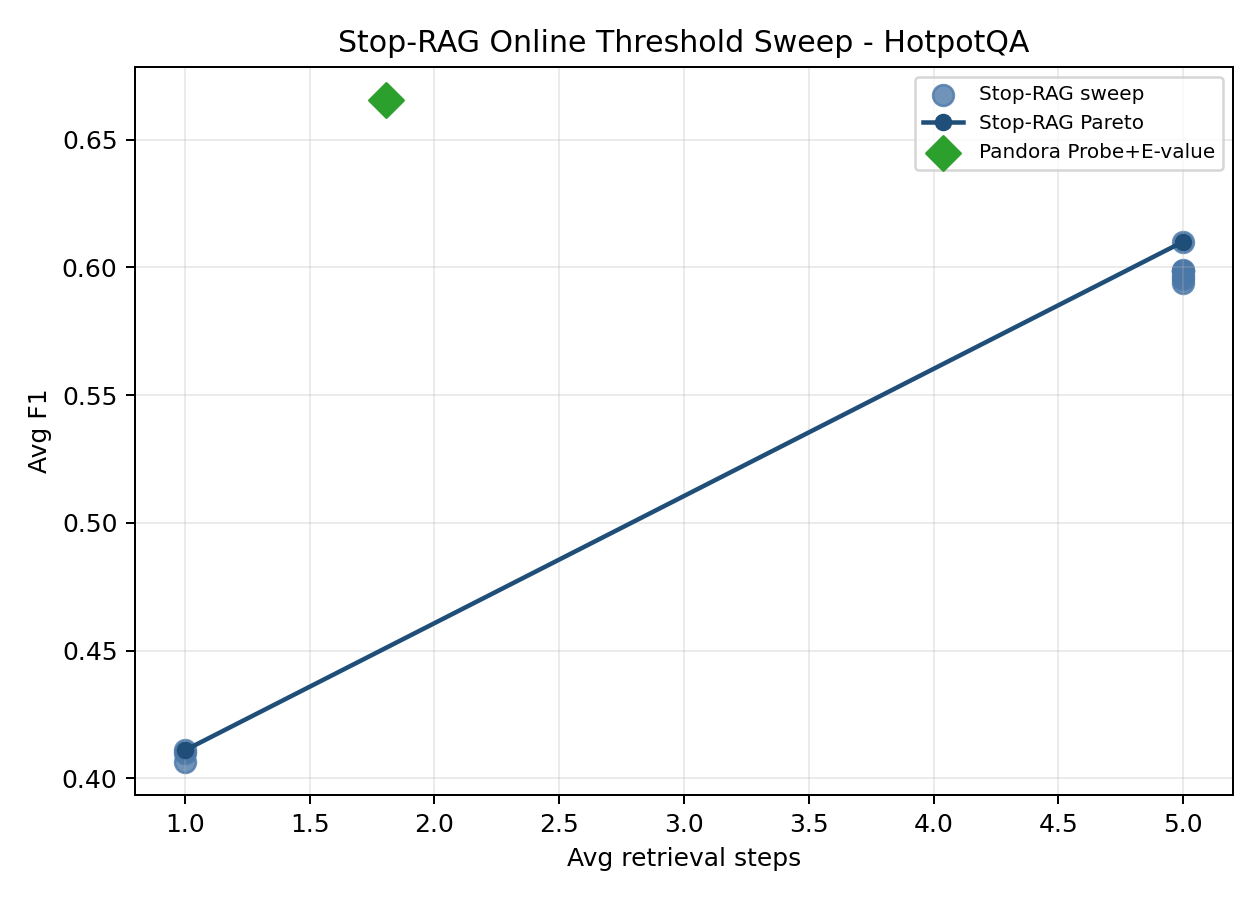
\includegraphics[width=0.32\linewidth]{results/stop_rag_pareto_hotpotqa.png}
  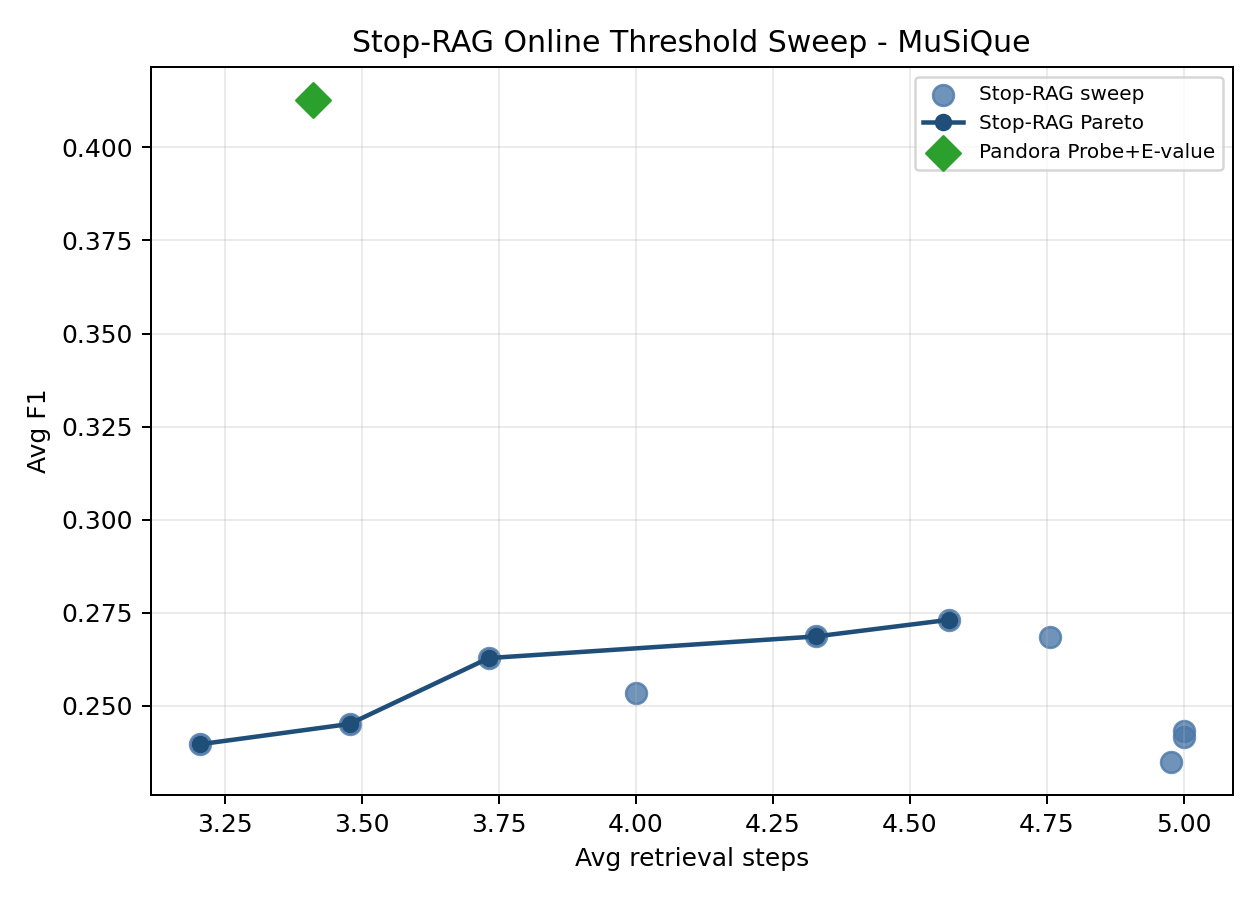
\includegraphics[width=0.32\linewidth]{results/stop_rag_pareto_musique.png}
  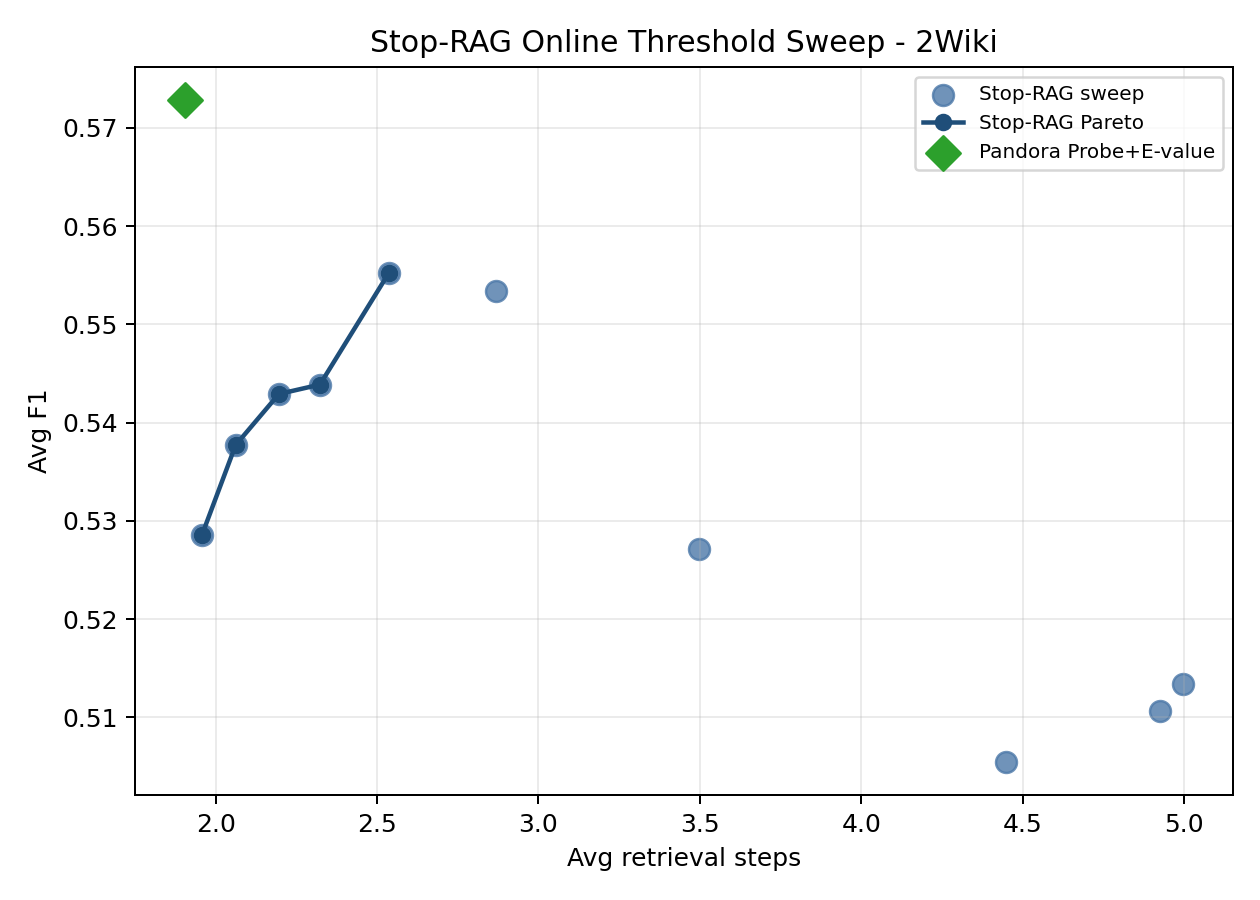
\includegraphics[width=0.32\linewidth]{results/stop_rag_pareto_2wiki.png}
  \caption{Aligned online fixed-checkpoint Stop-RAG threshold-sweep frontiers on \hotpot{}, \musique{}, and \twowiki{}. The sweep treats Stop-RAG as a Pareto baseline rather than a single-threshold comparison; \method{} Probe+E-value remains above the swept frontier on all three datasets.}
  \label{fig:stoprag}
\end{figure}

\section{Broader Impacts, Existing Assets, and Release Plan}
\label{app:assets}

\paragraph{Broader impacts.}
On the positive side, adaptive stopping can reduce retrieval cost and latency for multi-hop RAG systems, and the E-value layer adds a deployment-time warning signal for elevated risk rather than relying only on offline averages. This is particularly relevant for QA systems that may need to trade off answer quality, throughput, and cautious abstention under changing test streams.

Potential negative effects are also important. The monitor does not make the underlying system safe by itself: low-quality answers can still be produced before enough evidence accumulates, and a miscalibrated quality model could create a false sense of security. Selective prediction can also shift failure modes rather than eliminate them by refusing answers more often on high-risk inputs. Because the system is built on existing LLM and retrieval components, it inherits their factuality limits, representational biases, and licensing constraints. For this reason, we present the monitor as a diagnostic and intervention trigger, not as a guarantee that the stopped-answer stream is acceptable for high-stakes deployment.

\begin{table}[htbp]
  \caption{Asset-version-license summary for the anonymized paper bundle.}
  \label{tab:appendix-assets}
  \centering
  \scriptsize
  \setlength{\tabcolsep}{3pt}
  \begin{tabular}{>{\raggedright\arraybackslash}p{0.23\linewidth}>{\raggedright\arraybackslash}p{0.24\linewidth}>{\raggedright\arraybackslash}p{0.17\linewidth}>{\raggedright\arraybackslash}p{0.28\linewidth}}
    \toprule
    Asset & Version / identity & License / terms & Handling in supplement / release plan \\
    \midrule
    \hotpot{} & Project seed-42 manifest over the public benchmark release & Upstream benchmark terms & Not redistributed; the supplement ships only split manifests or manifest-generation instructions. \\
    \musique{} & MuSiQue v1.0 style benchmark files with the project seed-42 manifest & CC BY 4.0 & Not redistributed; the supplement ships only split manifests or manifest-generation instructions. \\
    \twowiki{} & Public 2Wiki release used by the project with the seed-42 manifest & Apache-2.0 & Not redistributed; the supplement ships only split manifests or manifest-generation instructions. \\
    Llama-3.1-8B-Instruct & \path{meta-llama/Meta-Llama-3.1-8B-Instruct} & Llama 3.1 Community License & Not redistributed; users obtain access separately under the terms of the upstream provider. \\
    Retriever / reranker models & \path{facebook/contriever-msmarco}; \path{BAAI/bge-reranker-v2-m3} & Upstream model / repo terms; Apache-2.0 for the reranker & Not redistributed; code paths are documented, but weights and indexes are obtained separately. \\
    Stop-RAG aligned baseline & Official Stop-RAG repository plus Pandora-authored alignment notes & Paper citation plus upstream repository terms; no clear public root software license is assumed here & The final public bundle excludes the copied comparison subtree and releases only Pandora-authored alignment notes, scripts, and evaluation summaries. \\
    Pandora-RAG code bundle & Anonymized method code in \texttt{pandora\_rag/} and \texttt{analysis\_tools/} & Apache-2.0 & Redistributed in the supplement with bundle-level \texttt{LICENSE} and \texttt{NOTICE}, while omitting checkpoints, caches, and credentials. \\
    Author-created paper figures & Figures authored for this paper & CC BY 4.0 & May be redistributed with the paper package. \\
    \bottomrule
  \end{tabular}
\end{table}

At submission time, we therefore distinguish between reproducibility support and public open access. The supplement can include the cleaned code bundle, deterministic split manifests or generation instructions, analysis scripts, and compact CSV/JSON summaries used to make the paper tables and figures. It does not need to redistribute benchmark data, model weights, copied baseline trees, or large cached artifacts. Any post-acceptance public release should preserve citations to the original datasets and baseline code, defer model access to the original providers, and include a license table aligned with the exact assets in the release package.

The release boundary is therefore explicit rather than implicit: Pandora-authored code and author-created figures can carry bundle-local licenses, while third-party datasets, model weights, and comparison assets remain under their upstream terms and are either excluded from redistribution or documented separately in the package notices. In particular, the final public bundle excludes the copied Stop-RAG comparison subtree and releases Pandora-authored Stop-RAG alignment notes instead.

\clearpage
\input{checklist}

\end{document}
